\documentclass{article}[18pt]
\usepackage{../../../../format}
\lhead{Theory of Computation - Algorithms and Complexity}


\begin{document}
\begin{center}
\underline{\huge Divide-and-Conquer Colouring for Restricted Inputs}
\end{center}
\section{Divide-and-conquer algorithms}
Many useful algorithms are recursive, i.e. call themselves recursively to deal with subproblems\\
\\
At each level of recursion:
\begin{itemize}
	\item \textbf{Divide} the problem into a number of subproblems
	\item \textbf{Conquer} the subproblems by solving them: recursively, or straightforward if the subproblem sizes are small enough
	\item \textbf{Combine} the solutions for the subproblems into a solution for the original problem 
\end{itemize}
\section{Problem Definition}
\begin{defin}[Colouring]
An assignment of colours to the vertices of a graph such that no two adjacent vertices get the same colour
\end{defin}

\begin{defin}[k-colouring]
	A colouring using at most k colours
\end{defin}
\begin{defin}[Chromatic number $\chi_G$]
	The smallest integer k for which G has a k-colouring
\end{defin}
The task of given a graph G determining $\chi_G$ is an NP hard problem
\section{How to deal with NP-hardness}
This can be done in several ways. For example:
\begin{itemize}
	\item Heuristics
	\item Approximation algorithms
	\item Exact algorithms
	\item Parametrized algorithms
	\item Algorithms with restricted inputs
\end{itemize}
We focus on the last approach. That is, we exploit the structure of the input with an aim to develop faster algorithms.\\
Justification
\begin{enumerate}
	\item In practice problem inputs may exhibit structure
	\item By focussing on the input structure we understand better what structure makes a problem computationally hard
\end{enumerate}
\section{Definition}
Let $G_1$ and $G_2$ be two vertex-disjoint graphs\\
\\
The \textbf{disjoint union} $G_1+G_2$ of $G_2$ and $G_2$ is the graph with the vertex set and edge set of the union of them. There is no overlap between $G_1$ and $G_2$\\
\\
The \textbf{join} $G_1\times G_2$ is the graph with vertex set $V(G_1)\cup V(G_2)$ and edge set $E(G_1)\cup E(G_2)\cup E^*$, where E* is the set of all edges between vertices of $G_1$ and vertices of $G_2$. Adding all possible edges between the graphs\\
A graph G is a cograph iff G can be created by the following rules
\begin{itemize}
	\item The 1-vertex graph $K_1$ is a cograph
	\item If $G_1$ and $G_2$ are cographs, then so is $G_1+G_2$
	\item If $G_1$ and $G_2$ are cographs, then so is $G_1\times G_2$
\end{itemize}
\begin{important}[Cographs]
	$P_4$ is the smallest graph that is not a cograph
\end{important}
\section{Alternate definition}
Let $P_4$ denote the path on 4 vertices\\
A graph G contains $P_4$ as an induced subgraph if G can be modified to $P_4$ via vertex deletions\\
If not, then G is said to be $P_4$-free
\begin{center}
	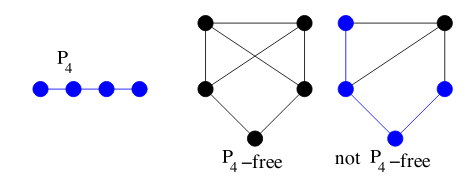
\includegraphics[scale=0.7]{p4}
\end{center}
It is known that a graph is a cograph iff it is $P_4$-free
\section{Definition of a cotree}
A cotree $T_G$ of a cograph G is the unique decomposition tree satisfying
\begin{enumerate}
	\item Its root r corresponds to the graph $G_r=G$
	\item Every left x of T corresponds to exactly one vertex of G, and vice versa
	\item Every internal node x of T has at least two children, is either labelled + of $\times$, and corresponds to an induced subgraph $G_x$ of $G$ defined as follows:
	\begin{itemize}
		\item If x is a +- node, then $G_x$ is the disjoint union of all graphs $G_y$, where y is a child of x
		\item If x is a $\times$-node, then $G_x$ is the join of all graphs $G_y$ where y is a child of x
	\end{itemize}
	\item Labels of internal nodes on the (unique) path from any leaf to r alternate between + and $\times$
\end{enumerate}
This tree shows the composition of a cograph, each internal node is an operation and each leaf is a vertex of the graph
\section{Solving colouring for cographs}
Let G be a cograph on n vertices and m edges\\
We construct its cotree $T_G$. This can be done in $\mathcal{O}(n+m)$ time\\
\\
We follow a bottum up approach: only process node x after first processing its children.\\
\\
Leaves: Each leaf corresponds to a single vertex of G. The chromatic number of a single-vertex graph is 1\\
\\
Union-nodes: Let x be a +-node. Then $\chi_{G_x}$ is the maximum number of the chromatic numbers of the graphs $G_y$, where y is a child of x\\
\\
Join-nodes. Let y be a $\times$-node. Then $\chi_{G_x}$ is the sum of the chromatic numbers of the graphs $G_y$, where y is a child of x\\
\\
In this way the last node we process is node r, which corresponds to the graph $G_r=G$\\
\\
As the number of nodes of T is $\mathcal{O}(n)$ and we used linear time per node, the total running time is polynomial
\end{document}